\documentclass[tikz,border=10pt]{standalone}
\usetikzlibrary{arrows.meta, positioning, calc}

\begin{document}
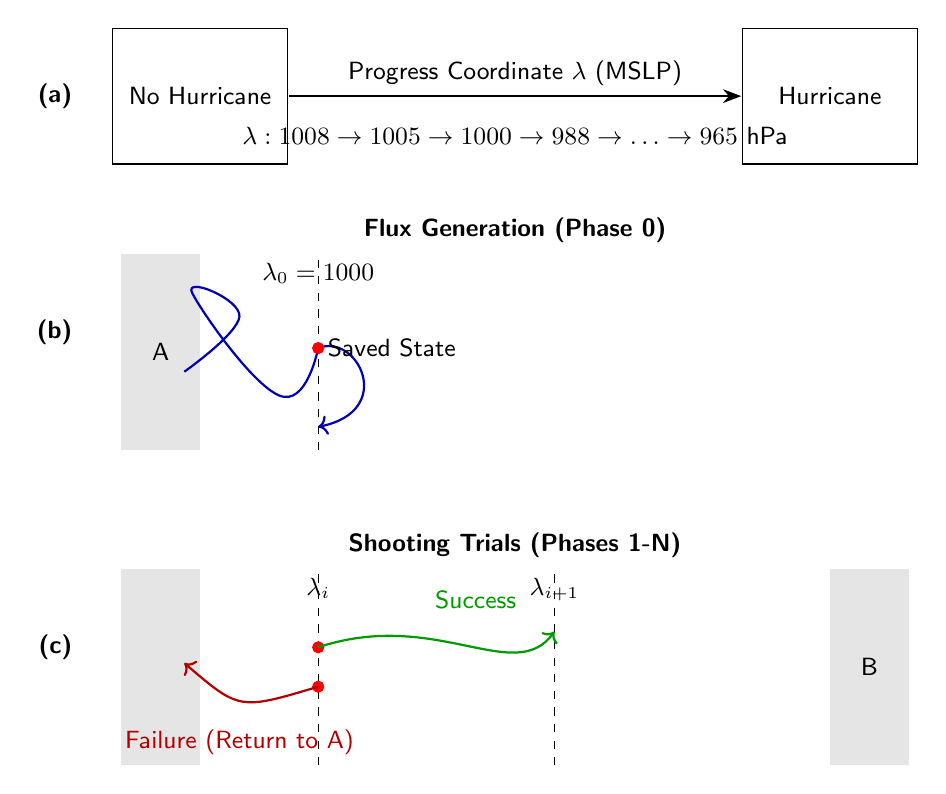
\begin{tikzpicture}[font=\sffamily\small]

% --- Panel (a): Concepts ---
\node[inner sep=0] (satA) at (-4, 4) {\fbox{\phantom{\rule{2cm}{1.5cm}}}}; % Placeholder for No Hurricane
\node at (-4, 4) {No Hurricane};
\node[inner sep=0] (satB) at (4, 4) {\fbox{\phantom{\rule{2cm}{1.5cm}}}}; % Placeholder for Hurricane
\node at (4, 4) {Hurricane};

\draw[thick, -{Stealth}] (satA) -- (satB) node[midway, above] {Progress Coordinate $\lambda$ (MSLP)};
\node at (0, 3.5) {$\lambda: 1008 \to 1005 \to 1000 \to 988 \to \dots \to 965$ hPa};
\node[left] at (-5.5, 4) {\textbf{(a)}};

% --- Panel (b): Flux Generation ---
\begin{scope}[yshift=0cm]
    \node[left] at (-5.5, 1) {\textbf{(b)}};
    \node at (0, 2.3) {\textbf{Flux Generation (Phase 0)}};
    
    % States
    \fill[gray!20] (-5, -0.5) rectangle (-4, 2);
    \node at (-4.5, 0.75) {A};
    
    % Interfaces
    \draw[dashed] (-2.5, -0.5) -- (-2.5, 2) node[below] {$\lambda_0 = 1000$};
    
    % Trajectory
    \draw[thick, blue!70!black] plot [smooth, tension=0.8] coordinates {(-4.2, 0.5) (-3.5, 1.2) (-4.1, 1.5) (-3, 0.2) (-2.5, 0.8)};
    \draw[thick, blue!70!black, ->] (-2.5, 0.8) .. controls (-2, 1) and (-1.5, 0) .. (-2.5, -0.2);
    
    % Checkpoints
    \filldraw[red] (-2.5, 0.8) circle (2pt) node[right, black] {Saved State};
\end{scope}

% --- Panel (c): Shooting ---
\begin{scope}[yshift=-4cm]
    \node[left] at (-5.5, 1) {\textbf{(c)}};
    \node at (0, 2.3) {\textbf{Shooting Trials (Phases 1-N)}};
    
    % States
    \fill[gray!20] (-5, -0.5) rectangle (-4, 2);
    \fill[gray!20] (4, -0.5) rectangle (5, 2);
    \node at (4.5, 0.75) {B};
    
    % Interfaces
    \draw[dashed] (-2.5, -0.5) -- (-2.5, 2) node[below] {$\lambda_i$};
    \draw[dashed] (0.5, -0.5) -- (0.5, 2) node[below] {$\lambda_{i+1}$};
    
    % Success Shot
    \filldraw[red] (-2.5, 1) circle (2pt);
    \draw[thick, green!60!black, ->] (-2.5, 1) .. controls (-1, 1.5) and (0, 0.5) .. (0.5, 1.2);
    \node[green!60!black] at (-0.5, 1.6) {Success};

    % Failure Shot
    \filldraw[red] (-2.5, 0.5) circle (2pt);
    \draw[thick, red!70!black, ->] (-2.5, 0.5) .. controls (-3.5, 0.2) .. (-4.2, 0.8);
    \node[red!70!black] at (-3.5, -0.2) {Failure (Return to A)};
\end{scope}

\end{tikzpicture}
\end{document}